\section{Viabilidade financeira}
O fato da aplicação ser \textit{\gls{open-source}} restringe a possibilidade de se ganhar dinheiro com venda direta, porém possibilita obtenção de lucro por meio de outras formas, como por exemplo:

\begin{itemize}
   \item \textbf{Utilização do servidor do fornecedor}: Nessa ocasião, a empresa contratante pagará um aluguel mensal para utilizar a aplicação hospedada no servidor do fornecedor;
   \item \textbf{Utilização de servidor próprio}: Utilização da aplicação em um servidor próprio da empresa contratante via pagamento de uma taxa de implementação mais uma de manutenção. Apesar de pagar mais pela implementação em um servidor próprio, a empresa contratante terá o direito de personalizar o produto de acordo com suas preferências nesse método de cobrança.
\end{itemize}

Há ainda a possibilidade de compilação independente do código-fonte da aplicação, por conta da premissa \textit{\gls{open-source}} citada anteriormente. Nesses casos, o fornecedor não se responsabilizará pela prestação de suporte.


Como forma de manter a aplicação, será cobrada uma taxa de R\$10,00 mensais da instituição de ensino por cada aluno que tiver acesso ao sistema, de modo a quitar o custo da implantação solicitada. Desse modo, os custos com hospedagem já estariam cobertos a longo prazo. A \autoref{tabela-previsao-orcamentaria} exibe uma previsão orçamentária para o projeto.

\begin{table}[htb]
\centering
\ABNTEXfontereduzida
\caption{\label{tabela-previsao-orcamentaria} Previsão orçamentária mensal do Projeto Turma de Elite}
\begin{tabular}{|p{2.5cm}|c|c|c|c|c|}
   \hline
   \thead{} & \thead{100 alunos}  & \thead{1000 alunos}  & \thead{5000 alunos} & \thead{10000 alunos} & \thead{50000 alunos} \\\hline
   Heroku & R\$127* & R\$506* & R\$1010* & R\$5048* & R\$10096*  \\\hline
   Heroku Postgres & R\$252* & R\$1764* & R\$3780* & R\$12600* & R\$30240*  \\\hline
    Firebase Hosting & R\$0 & R\$177* & R\$411* & R\$832* & R\$5689* \\\hline
    Firebase Authentication & R\$0 & R\$0 & R\$0 & R\$3029* & R\$18172* \\\hline
    Receita & R\$1000 & R\$10000 & R\$50000 & R\$100000 & R\$500000 \\\hline
    Lucro & R\$621 & R\$7553 & R\$44799 & R\$78491 & R\$435803\\\hline
\end{tabular}
\fonte{Dados do Projeto}
\legend{* - O valor exibido foi aproximado com base na cotação do dólar americano para o dia 08/06/2021 (US\$1 = R\$5,04)}
\end{table}
\FloatBarrier

Com relação aos \textit{\glspl{dyno}} do \textit{Heroku} para hospedar a quantidade crescente de acessos concorrentes, a relação obtida foi:
\begin{itemize}
    \item \textbf{100 alunos}: 1 \textit{\gls{dyno}} - \textit{Standard} 1X;
    \item \textbf{1000 alunos}: 2 \textit{\glspl{dyno}} - Standard 2X;
    \item \textbf{5000 alunos}: 4 \textit{\glspl{dyno}} - Standard 2X;
    \item \textbf{10000 alunos}: 4 \textit{\glspl{dyno}} - Performance M;
    \item \textbf{50000 alunos}: 2 \textit{\glspl{dyno}} - Performance L.
\end{itemize}

A \autoref{fig:precos-heroku} apresenta as relações de preço presentes no website do Heroku.

\begin{figure}[htb]
    \centering
	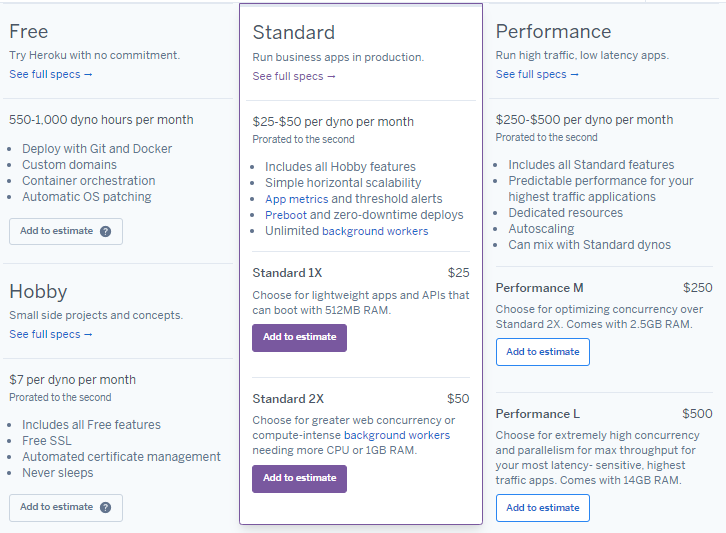
\includegraphics[width=16cm]{imagens/precos-heroku.png}
	\caption{\label{fig:precos-heroku} Preço mensal de aluguel dos \textit{\glspl{dyno}} do Heroku}
	\fonte{\cite{heroku:2021}}
\end{figure}

O custo de hospedagem do \textit{\gls{front-end}} e autenticação variou conforme a quantidade de armazenamento e suporte a acessos simultâneos necessários para atender a quantidade crescente de alunos.

Para a hospedagem do banco de dados será utilizado o Heroku Postgres. Para cada demanda de usuários será utilizado um plano diferente do Heroku Postgres, onde os planos oferecem diferentes quantidades de memória \ac{ram}, armazenamento e acessos simultâneos. Durante a etapa de desenvolvimento será utilizado o plano "Hobby Dev", que é gratuito. Já durante o funcionamento da aplicação será utilizado um plano diferente, visto que cada plano oferta diferentes quantidades de recursos e possuem diferentes valores. Portanto, cada plano será utilizado para atender adequadamente a demanda de usuários.

\begin{itemize}
    \item \textbf{100 alunos}: Standard 0 (4 GB de \ac{ram}, 64 GB de armazenamento e 120 conexões simultâneas por US\$50 mensais);
    \item \textbf{1000 alunos}: Premium 0 (4 GB de \ac{ram}, 64 GB de armazenamento, 120 conexões simultâneas e alta disponibilidade por US\$200 mensais);
    \item \textbf{5000 alunos}: Premium 2 (8 GB de \ac{ram}, 256 GB de armazenamento e 400 conexões simultâneas US\$350 mensais);
    \item \textbf{10000 alunos}: Premium 4 (30.5 GB de \ac{ram}, 1 TB de armazenamento, 500 conexões simultâneas e alta disponibilidade por US\$1200 mensais);
    \item \textbf{50000 alunos}: Premium 7 (244 GB de \ac{ram}, 2 TB de armazenamento, 500 conexões simultâneas e alta disponibilidade por US\$6000 mensais).
\end{itemize}